\documentclass[runningheads,a4paper]{llncs}
\usepackage{amssymb}
\setcounter{tocdepth}{3}
\usepackage{graphicx}
\usepackage{epstopdf}
\usepackage{url}
\usepackage{array}
\usepackage{multirow}
\usepackage{array}
\usepackage{caption} 
\newcolumntype{L}[1]{>{\raggedright\let\newline\\\arraybackslash\hspace{0pt}}m{#1}}
\newcolumntype{C}[1]{>{\centering\let\newline\\\arraybackslash\hspace{0pt}}m{#1}}
\newcolumntype{R}[1]{>{\raggedleft\let\newline\\\arraybackslash\hspace{0pt}}m{#1}}
\captionsetup[table]{skip=10pt}
\urldef{\mailsa}\path|{1212069,1212304}@student.hcmus.edu.vn, nqminh@fit.hcmus.edu.vn|

\newcommand{\keywords}[1]{\par\addvspace\baselineskip
\noindent\keywordname\enspace\ignorespaces#1}


\begin{document}

\mainmatter

% Title của paper
\title{Aspect-based Sentiment Analysis using \\ Word Embedding Restricted Boltzmann Machines}
% a short form should be given in case it is too long for the running head
\titlerunning{Aspect-based Sentiment Analysis using Word Embedding RBM}
% Authors

\author{Bao-Dai Nguyen-Hoang
\and Quang-Vinh Ha
\and Minh-Quoc Nghiem}


% Nơi làm việc công tác
% Không cung cấp địa chỉ email nếu chưa được nhận đăng bài
\institute{Faculty of Information Technology\\
	Ho Chi Minh City University of Science\\
	227 Nguyen Van Cu St., Ward 4, District 5, Ho Chi Minh City, Vietnam\\
\mailsa
}

%
% NB: a more complex sample for affiliations and the mapping to the
% corresponding authors can be found in the file "llncs.dem"
% (search for the string "\mainmatter" where a contribution starts).
% "llncs.dem" accompanies the document class "llncs.cls".
%

\maketitle


\begin{abstract}
Recent years, many studies have addressed problems in sentiment analysis at different levels, and building aspect-based methods has become a central issue for deep opinion mining.
However, previous studies need to use two separated modules in order to extract aspect-sentiment word pairs, then predict the sentiment polarity.
In this paper, we use Restricted Boltzmann Machines in combination with Word Embedding model to build the joined model which not only extracts aspect terms appeared and classifies them into respective categories, but also completes the sentiment polarity prediction task.
The experimental results show that the method we use in aspect-based sentiment analysis tasks is better than other state-of-the-art approaches.

\keywords{Aspect-based, Sentiment Analysis, Opinion Mining, Restricted Boltzmann Machine, Supervised Learning, Word Embedding}
\end{abstract}


\section{Introduction} \label{introduction}
% Giới thiệu bài toán Sentiment Analysis
Sentiment Analysis (also known as opinion mining) is the process of determining whether a piece of writing is positive or negative.
With the development of opinionated user-generated review sites, many customers can write reviews and express their opinions about the products (or services).
Sentiment Analysis could help not only users to choose the right products but also companies to improve their products based on these reviews.

% Giới thiệu bài toán AB Sentiment Analysis, joint model
Aspect-based Sentiment Analysis (ABSA) has received much attention in recent years since each review might contain many aspects.
For example, in a restaurant review, we may have opinions about \textit{food}, \textit{staff}, \textit{ambience}, etc.
Conventional ABSA systems normally have two separated modules: one for aspect extraction and another one for sentiment classification~\cite{bingliu,google,WebUserAnalysis_kumar}.
Recently, Wang et al.~\cite{serbm} introduced a joint model, called Sentiment-Aspect Extraction based on Restricted Boltzmann Machines (SERBM), that extract aspects and classify sentiments at the same time.
In this model, they used unsupervised Restricted Boltzmann Machine~(RBM) and three different types of hidden units to represent aspects, sentiments, and background information, respectively.
Furthermore, they added prior knowledge into this model to help it acquire more accurate feature representations.
The visible layer $\textbf{v}$ of SERBM is represented as a $K \times D$ matrix, where $K$ is the dictionary size and $D$ is the document length.
They showed that their model is well-suited for solving aspect-based sentiment analysis tasks.

% research gap
However, there are two main problems still exist in the SERBM model.
Firstly, an unsupervised method can only cluster reviews into categories and we can not know the name of the category.
No information was given to determine which position of the hidden units to represent aspects, sentiments or background words during the training process.
Secondly, a visible layer will be a matrix combined by high-dimensional vectors if training data has a large set of vocabulary, which requires much computational resource.

% Proposed
In this paper, we propose combining Restricted Boltzmann Machine with Word Embedding model to overcome the limitations of existing method.
Word Embedding model has the capability of reducing the dimensionality of the input vectors.
Therefore, we can use it to reduce the dimensionality of the input in visible layer while keeping the semantics of the reviews.
We encode the input document as a vector, created by the Word Embedding model, instead the vector of one-hot encoding Bag Of Words model.
Furthermore, we use RBM in a supervised setting.
We move the output component from hidden layer to visible layer.
The hidden layer now acts as the dependencies between the components in the visible layer.
Doing like this, we can fix the units for desired categories.

We call our model Word Embedding Restricted Boltzmann Machine (WE-RBM).
Overall, our main contributions are as follows:
\begin{itemize}
\item This is the first work that combines Word Embedding model and supervised RBM for the ABSA task. Compared with other state-of-the-art methods, our model can identify aspects and sentiments efficiently, yielding 1-6\% improvements in accuracy for sentiment classification task and 1.73\% to 7.06\% improvements in F1 score for aspect extraction task.
\item By using Word Embedding model, we can efficiently reduce the size of input vectors up to 100 times, which in turn reduces the training time greatly.
\item We also introduce a simple yet efficient way to incorporate prior knowledge into RBM model. Prior knowledge is the advantage of Word Embedding model, which can help RBM to be well-suited for solving aspect-based opinion mining tasks.
\end{itemize}

% Format of the paper
The rest of this paper is organized as follows.
Section~\ref{related-work} introduces the related work.
Section~\ref{proposed-method} overviews the background information, then describes our approach to classify reviews into aspect categories and predict sentiment polarity of the reviews.
Experimental results are presented in Section~\ref{experiments}.
Finally, Section~\ref{conclusion} concludes the paper and discusses future work.

% The results obtained based on the dataset of reviews in restaurant domain, which widely adopted by previous work~\cite{data_ganu,Brody_Elhadad,Zhao} (Ganu et al., 2009; Brody and Elhadad, 2010; Zhao et al., 2010).

%Therefore, new customers may find it difficult to explore the large number of reviews in order to make right decision, since many people have different purposes, which base on different aspects of the product.

% These two parts are analyzing opinionated texts, such as opinions, sentiments by extracting the aspect-term appeared in the sentences, and classifying them into two classes (positive or negative).
% It helps people make the right decisions thanks to the fine-grained analysis on each aspect of the products.
% In previous work, Liu and Hu~\cite{bingliu,google,WebUserAnalysis_kumar} proposed combining two or more modules to complete the ABSA model.
% For instance, we can use one for extracting aspect-sentiment word pairs, one for sentiment prediction, another optional module is to summarize the opinions.

% giving a brief synopsis of the relevant literature
% Some work has been investigated to extract the candidate product feature opinion pairs.
% Kumar and Raghuveer~\cite{WebUserAnalysis_kumar} use the rules on the typed dependency tree, then they use lexicons to classify and generate a summary of the product.
% In Toh and Wang~\cite{Toh_and_Wang}, they build a Conditional Random Field (CRF) based classifier for Aspect Term Extraction and a linear classifier for Aspect Term Polarity Classification, but there is no method to extract the opinion words in the sentences.
% Unsupervised method such as Latent Dirichlet Allocation (Blei et al., 2003)~\cite{LDA_Blei} is also used to extract and group corresponding representative words into categories.
% Such approaches, however, must use two-separated modules to perform both aspect extraction and sentiment classification, or just only have ability to solve one of these tasks.

% research gap
% Hence, Wang et al.~\cite{serbm} adapted the Sentiment-Aspect Extraction based on Restricted Boltzmann Machines (SERBM) to overcome this problem.
% Three different types of hidden units are used to represent aspects, sentiments, and background words in this model, respectively.
% Furthermore, they blend background knowledge into this model using priors and regularization to help it acquire more accurate feature representations.
% The visible layer $\textbf{v}$ of SERBM is represented as a $K \times D$ matrix, where $K$ is the dictionary size and $D$ is the document length, or the number of sentences in reviews.
% However, much uncertainty still exists about the defined hidden units in hidden layer.
% First, unsupervised method can just cluster reviews into categories and can not fix the unit for desired category.
% No information given to determine which position of the hidden units to represent aspects, sentiments or background words during the training process.
% Second, visible layer would be a matrix combined by high-dimensional vectors if training data set had varied vocabulary, which result in insufficient computational resources.

% My work and paper format
% In this paper, we implement Vector Space model combined with Restricted Boltzmann Machine (VS-RBM) to extract aspect term appeared and classify sentiment polarity of the sentences.
% The reasons we propose VS-RBM include the ability to jointly model aspect and sentiment information together and the capability in reducing dimensionality of the input vectors.
% In this two-layer structure model, we do not use hidden layer as output layer but the dependencies between the components of observations in visible layer.
% Each input unit in the visible layer is a component of the feature vector, created by the Vector Space Model instead of using the Bag Of Words model as previous approach.
% This helps reduce the dimensionality of the input while keeping documents' semantics.
% The results obtained based on the dataset of reviews in restaurant domain, which widely adopted by previous work~\cite{data_ganu,Brody_Elhadad,Zhao} (Ganu et al., 2009; Brody and Elhadad, 2010; Zhao et al., 2010).



\section{Related work} \label{related-work}

ABSA approaches may be divided into three main categories: rule-based, supervised learning, and unsupervised learning.

% Rule-based
Rule-based approaches~\cite{bingliu,Ding} can perform quite well in a large number of domains.
They use a sentiment lexicon, expressions, rules of opinions, and the sentence parse tree to help classify the sentiment orientation on each aspect appeared in a review.
They also consider sentiment shifter words (i.e. \textit{not}, \textit{none}, \textit{nobody}, etc.).
However, these rule-based methods have a shortcoming in processing complex documents where the aspect is hidden in the sentence, and failing to group extracted aspect terms into categories.

% Supervised AE + SC
For the supervised learning approach, Wei and Gulla~\cite{Wei_Gulla} propose a hierarchical classification model to determine the dependency and the other relevant information in the sentence.
Jiang et al.~\cite{Jiang}, Boiy and Moens~\cite{Boiy} use dependency parser to generate a set of aspect-dependent features for classification, which weighs each feature based on the position of the feature relative to the target aspect in the parse tree.
Several other supervised learning models have been published, such as Hidden Markov Models~\cite{Jin_Wei}, SVMs~\cite{ABSA_SVM}, Conditional Random Fields~\cite{Choi_Yejin,Jakob_Iryna}.

% Unsupervised AE + SC
% Joint model
It has been demonstrated that a classifier trained from labeled data in one domain often performs poorly in another domain~\cite{BingLiubooks}.
Hence, unsupervised methods are often adopted to avoid this issue.
Several recent studies investigate statistical topic models which are unsupervised learning methods.
They assume that each document consists of a mixture of topics.
Specifically, Latent Dirichlet Allocation (LDA)~\cite{LDA_Blei}, Multi-Grain LDA model~\cite{Titov_Ryan} are used to model and extract topics from document collections.
A number of authors have considered the effects of topic models on ABSA task, such as the two-step approach~\cite{Brody_Elhadad}, joint sentiment/topic model~\cite{Lin_He}, and topic-sentiment mixture model~\cite{Mei}.
A recent study by Wang et al.~\cite{serbm} proposed the SERBM model which also jointly address these two tasks in an unsupervised setting.
% The two-step approach by Brody and Elhadad~\cite{Brody_Elhadad} to detect aspect-specific opinion words includes identifying aspects using topic models and identifying aspect-specific sentiment words by considering adjectives only.
% The joint sentiment/topic model was proposed by Lin and He~\cite{Lin_He} to separate aspect words and sentiment words.
% Mei et al.~\cite{Mei} proposed the topic-sentiment mixture model based on three separated models with the help of some external training data is proposed to extract aspect and sentiment words.

%Supervised learning is dependent on the training data and has difficulty to scale up to a large number of application domains.




\section{Proposed method}\label{proposed-method}
\subsection{Background}
\subsubsection{Restricted Boltzmann Machine}

RBM model, a generative stochastic artificial neural network, is treated as a model in the field of deep learning.
RBM can be used to learn important aspects of an unknown probability distribution based on samples from this distribution~\cite{Fischer2012}.
Recently, researchers have applied RBM in the field of Natural Language Processing, including topic modeling and sentiment analysis~\cite{serbm}.
One special characteristic of RBM is that it can be used in both supervised and unsupervised ways, depending on the task.

As shown in Figure~\ref{fig:rbm1}, RBM model is a two-layer neural network which contains one visible layer and one hidden layer.
The visible layer is constituted by visible units correspond to the components of an observation (e.g., one visible unit for each word in an input document).
The hidden layer composed of hidden units which model the dependencies between the components of observations (e.g., dependencies between words in the document).

\begin{figure}
	\centering
	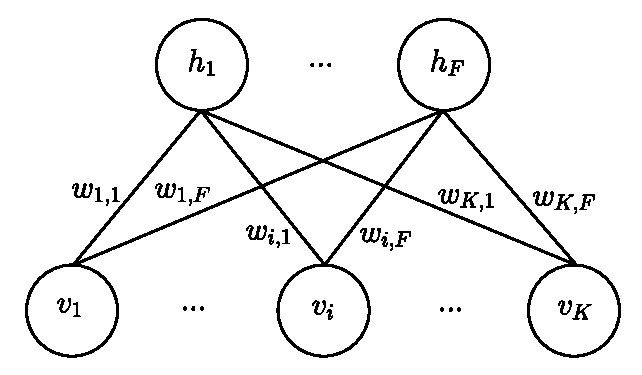
\includegraphics[height=3cm]{BasicRBM}
	\caption{The network graph of an RBM model with $K$ visible and  $F$ hidden units}
	\label{fig:rbm1}
\end{figure}

\subsubsection{Word Embedding model}

% Gioi thieu Word2Vec
The Word Embedding model (WEM) is a proven and powerful paradigm in Natural Language Processing, in which words are represented as vectors in a high-dimensional space~\cite{Quoc_Le}.
The idea of this model is representing words as vectors.
Therefore, the similarity of two words $i$ and $j$ can be calculated based on the cosine of the angle between the vectors as shown in equation~\ref{cosine_equal}.

\begin{equation} \label{cosine_equal}
\cos\theta=\frac{w_i.w_j}{||w_i|| ||w_j||}
\end{equation} 

where $w_i.w_j$ is the dot product of these two documents while $||w_i||$ and $||w_j||$ are the norm of vector $w_i$ and $w_j$, respectively.

% Mo rong Word2Vec thanh Doc2Vec
For document representation, every word appeared in the document is represented as a vector.
We then sum all of these vectors to get a vector that represent the document~\cite{Quoc_Le}.

\subsection{Our Aspect-based Sentiment Analysis model}
% Giới thiệu mô hình

\subsubsection{Structure}

% Research gap: fixed hidden unit
In the previous approach, Wang et al.~\cite{serbm} proposed an unsupervised RBM model to ABSA.
As mention before, there are two main shortcomings in this SERBM model.
%Although this model can help to overcome the limitations of hand-labeled training data, but there still exist certain shortcomings.
Firstly, an unsupervised method can only cluster reviews into categories and we can not know the name of the category.
This model fixes hidden units 0--6 to represent the target aspects \textit{Food}, \textit{Staff}, \textit{Ambience}, \textit{Price}, \textit{Ambience}, \textit{Miscellaneous}, and \textit{Other Aspects}, respectively.
%This may reduce the accuracy of the classification.
%Since unsupervised learning model can not fix the categories which it will cluster into the output units.
There is no way we can determine the aspects (e.g. which unit represents \textit{Food}, which unit represents \textit{Staff}) based on the position of the hidden units alone.

% Reseach gap: size of vector
Secondly, when training, each document is transformed into a $ \textit{K} \times \textit{D} $ matrix $\textbf{v}$, where $\textit{K}$ is the dictionary size, and $\textit{D}$ is the document length.
If visible unit $\textit{i}$ in $\textbf{v}$ takes the $\textit{k}$-th value, $v^k_i$ is set to 1.
If the training data has a large set of vocabulary, the visible layer will be a matrix combined by high-dimensional vectors.
These sparse input vectors lead to not only the decrease in the model's accuracy but also the increase in computational resources.

% Giải quyết research gap, sơ lược mô hình
To overcome these problems, we propose a method using supervised RBM model which is illustrated in Figure~\ref{fig:rbm2}.
The \textbf{\textit{Output units}} include the units represent the aspects and sentiment orientations of the reviews.
We call them \textit{Aspects identifying units} and \textit{Sentiments identifying units}, respectively.
These units are put together with \textbf{\textit{Input units}} in the visible layers, instead of being placed in hidden layers.
Meanwhile, the units in the hidden layer represent the relationship between the units in the visible layers.
We encode input units in the visible layer as a vector, created by the Word Embedding model~\cite{rehurek_lrec_word2vec}, instead the vector of one-hot encoding Bag Of Words model.
This helps reduce the dimensionality of the input matrix while keeping documents' semantics.

\begin{figure}
	\centering
	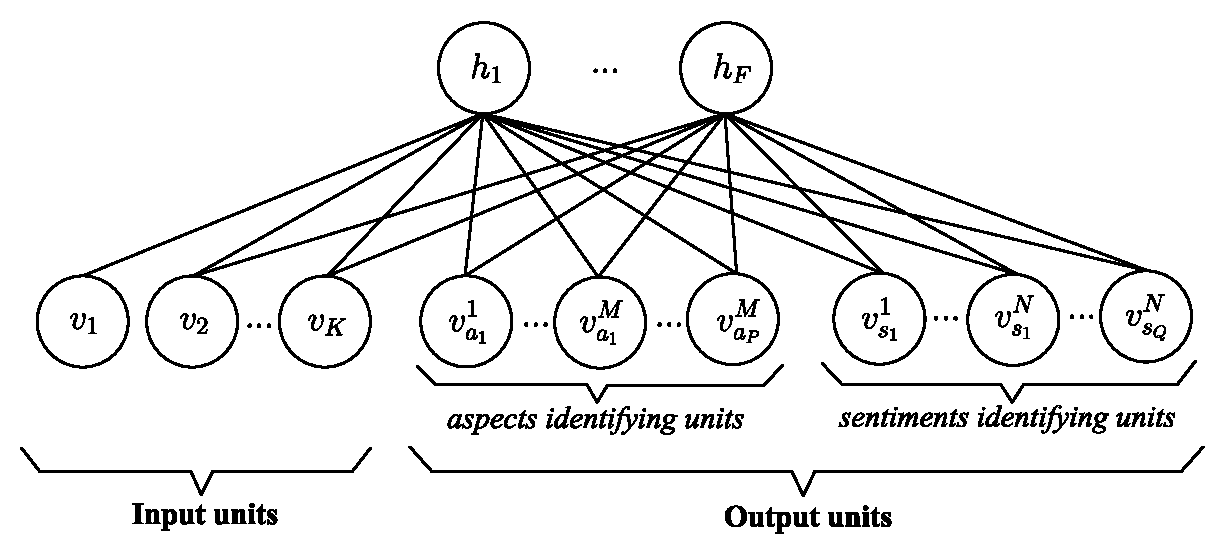
\includegraphics[height=4.5cm]{SupervisedRBM}
	\caption{The network graph of our Supervised Sentiment-Aspect Extraction RBM model}
	\label{fig:rbm2}
\end{figure}

% Nói chi tiết điểm khác biết giữa RBMs bình thường, chức năng mỗi node
Compared to standard RBMs, the first difference of this model is the visible layer.
Apart from the input units, there are also aspect and sentiment identifying units that represent the output component of the model.
Suppose in the training data, there are reviews talking about $P$ aspects and having $Q$ sentiment orientations in total.
In particular, the set of aspects is $ A = \{a_1, a_2, ..., a_P\}$, and the set of sentiment orientations is $ S = \{s_1, s_2, ..., s_Q\}$.

For each aspect, the model set $M$ units to capture that aspect.
For example, if the review mentioned aspect $a_i \in A$, we set the units from $v^1_{a_i}$ to $v^M_{a_i}$ to 1, and 0 otherwise.
We use the same setting for sentiment units.
The model set $N$ units to capture each sentiment polarity.
If the sentiment polarity is $s_j \in S$, we set the units from $v^1_{s_j}$ to $v^N_{s_j}$ to 1, and 0 otherwise.
The idea of setting M and N units to capture aspects and sentiment polarity is obtained from previous work~\cite{Fischer2012}.
Our model has the property that input units and output units stay in the same layer.
If we used only one output unit for each aspect and sentiment polarity while there are too many input units, the model would be imbalance and need more time to converge. 

% Nêu lý do tại sao lại chọn mô hình này
With this structure, our model can solve two tasks simultaneously: aspect identification and sentiment classification.
This ability of our model is reflected in the aspect and sentiment identifying units which play important roles in the sampling process of RBM.
Meanwhile, weight values of connecting edges contain semantic information of the review, which help identifying units to communicate with the hidden layer.
In addition, the fixed dimension of the input vector does not depend on the number of vocabulary words.
This capability not only helps the model prevent the occurrence of decreasing speed and accuracy, but also solves the semantic problem in the review.

For the customer restaurant reviews analyzing task, one word in a review may mention a certain aspect (e.g. ``delicious" corresponds to \textit{food} aspect), or a certain opinion (e.g. ``good" is about positive sentiment, while ``bad" is about negative sentiment).
Furthermore, there are other words do not mention about aspect or sentiment, they can be removed during the preprocessing phase.
These latent topics in a review are considered as the factors which generate aspect and sentiment words within that review.
To technically illustrate this, hidden layer contains information of the latent topics.
In the generation process, hidden units produce the values of visible units, which are also the information of the aspect and sentiment words in reviews.
Moreover, we can increase the number of hidden units in order to increase the modeling capacity of the RBM, which make the model powerful enough to represent complicated distributions.

\subsubsection{Word Embedding Restricted Boltzmann Machine}

% Những bất cập khi sử dụng chỉ word2vec mà không có prior knowledge
When we use supervised RBM with input vectors generated by Word Embedding model, the results showed that RBM does not have enough capacity to regenerate visible units.
Much of the instability in this approach stems from two reasons. 
Firstly, RBM has only hidden and visible layers to capture the diversity of semantic of documents.
Secondly, in visible and hidden units, the values vary continuously by each epoch in the training process.
This leads to loss of semantic information of documents.
One way to solve this problem is increasing the number of hidden units for RBM to accommodate more information.
However, increasing the number of hidden units causes the model to increase the number of visible units.
This leads to the problem encountered in the previous approach~\cite{serbm}, which is insufficient computational resources.

% Đề xuất thêm mô hình WE-RBM sử dụng prior knowledge
Therefore, we propose Word Embedding Restricted Boltzmann Machine (WE-RBM) to take full advantage of WEM's structure and supervised RBM.
Beside input units, WE-RBM also uses prior knowledge obtained from the vector comparing process of WEM.
Hence, the model would have more information to make up for the loss in the training process.
Our WE-RBM model is expressed in Figure~\ref{fig:vs-rbm}.

% Hình figure của WE-RBM
\begin{figure}
	\centering
	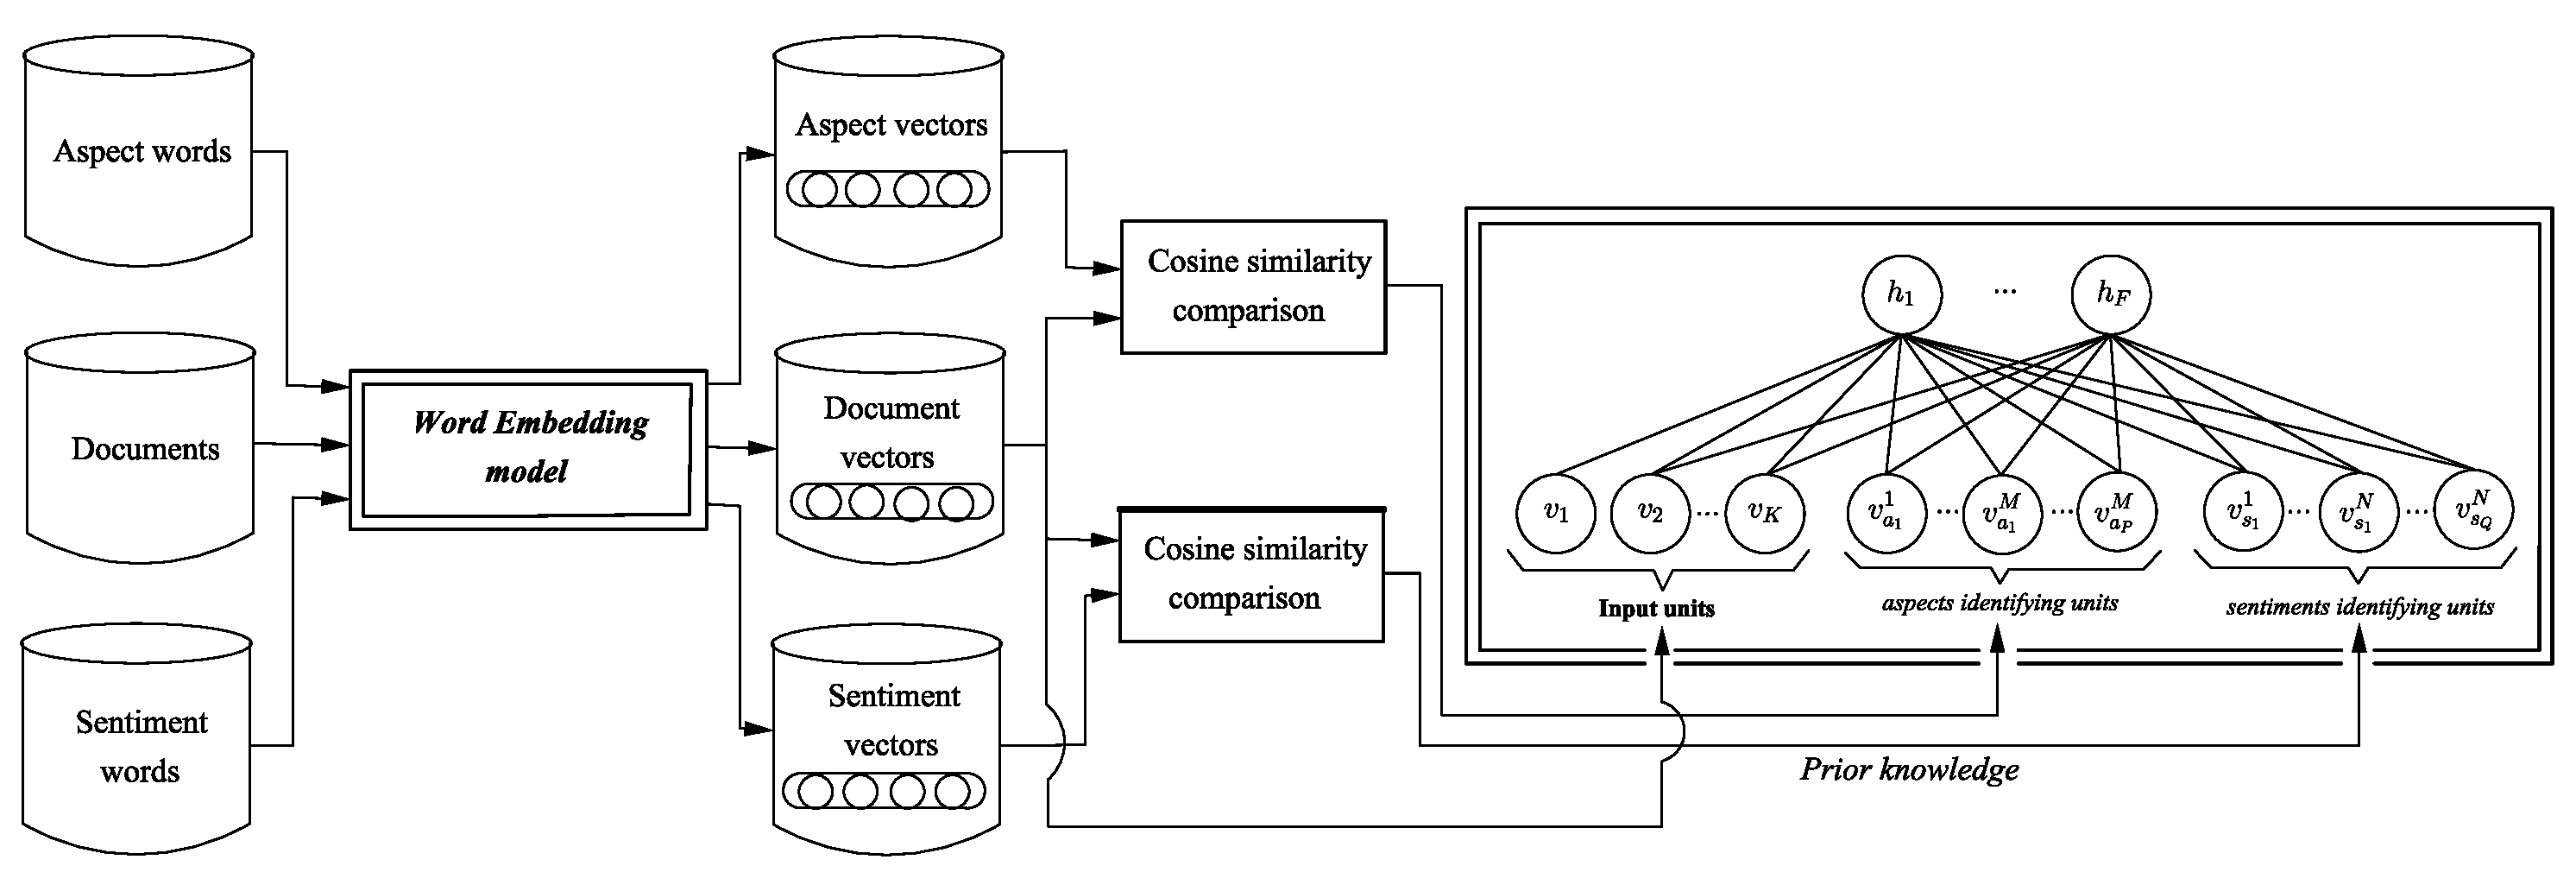
\includegraphics[height=4.0cm]{WE-RBM}
	\caption{WE-RBM model overview. Double boxed items are main components in WE-RBM model.}
	\label{fig:vs-rbm}
\end{figure}

% Giải thích figure
% Quá trình train
Assuming that WEM has been trained independently before, we put every document into WEM to generate the corresponding vector.
The dimension of each vector is equal to the number of input units of RBM.
After document vectors generation process, we make the training phase for the RBM model in a supervised setting.
This phase helps the model be able to understand the vectors' pattern generated by WEM.

% Trong quá trình test
In the testing phase, each document is also converted into a vector by WEM.
Unlike previous work, the aspect identification and sentiment classification task are firstly performed by WEM instead of RBM model.
Particularly, WE-RBM computes the cosine similarity score (shown in equation \ref{cosine_equal}) between the document vector and each of all aspect and sentiment vectors, which are also generated by WEM.
The prior knowledge is determined by the highest similar pair of vectors.

For instance, a document $d$ can be categorized into one of these aspects $S = {a_1, a_2,..., a_P}$.
Let us call the vector form of document or aspect $x$ $vec(x)$.
Prior knowledge would be labeled $i$ if cosine similarity between $vec(d)$ and $vec(a_i)$ is the highest one.
The model performs similarly with sentiment classification task.
This prior knowledge can help improve the ability of the model to extract aspects and identify sentiments.
 
% Lý do có được ý tưởng này
One characteristic of WEM is two vectors which represent two different words would have high cosine similarity if these two words have close meaning to each other~\cite{rehurek_lrec_word2vec,Milokov_word2vec} (e.g. ``strong" may have close meaning with ``powerful", whereas ``strong" and ``London" are more distant).
Inspired by this, we use WEM to categorize aspect and classify sentiment before feeding the input vector into RBM model.
Hence, each document can have its own prior knowledge before RBM's classification.
The final classification result is determined by both WEM and RBM.
Therefore, we call our novel combination model is WE-RBM.

% Giải thích tại sao lựa chọn mô hình này, lợi ích của mô hình
There are three main reasons we propose this novel WE-RBM model to solve the ABSA's tasks.
Firstly, when a document is converted into vector form, it can be compared with other documents by cosine similarity while semantic information is conserved.
This is the advantage of word representation technique that WE-RBM use in the classification process.
Secondly, WE-RBM can save computational resources and processing time.
The model does not need to adapt input units for huge dictionary size thanks to fixed dimension of the input vector.
Using prior knowledge instead of increasing hidden units, WE-RBM can handle big training set in reduced processing time.
Last but not least, our WE-RBM model also has the capability of jointly modeling aspect and sentiment information together.

\subsubsection{Training and Testing}
% Mô tả quá trình huấn luyện của mô hình
In the training process, Contrastive Divergence (CD), also called Approximate Gradient Descent, is the way that helps RBM learn the connection weights in the network.
CD has two phases, which are Positive phase and Negative phase.
In each phase, we compute the positive and negative value by the multiplication of visible and hidden units.
Then, we update the connection weight based on the subtraction from positive value of negative value.
Particularly, each epoch of CD can be expressed in five steps below:

\textbf{\emph{Step 1}}.
Update the states of the hidden units using the logistic activation rule described in equation~\ref{equation:vtoh}.
For the $j$-th hidden unit, compute its activation energy and set its state to 1 with corresponding probability.
\begin{equation} \label{equation:vtoh}
P(\emph{h}_j=1| \textbf{v})=sigm(a_j+\sum^D_{i=1}\sum^K_{k=1}v^k_iW^k_{ij})
\end{equation}

\textbf{\emph{Step 2}}.
For each connection edge $e_{ij}$, get the value from positive phrase by equation~\ref{pos_phrase}.
\begin{equation} \label{pos_phrase}
pos(e_{ij}) = v_ih_j
\end{equation}

\textbf{\emph{Step 3}}.
Reconstruct the visible units in a similar manner by using the logistic activation rule described in equation~\ref{equation:htov}.
For the $i$-th visible unit, compute its activation energy and set its state to 1 with corresponding probability.
Then do \textbf{\emph{Step 1}} to update the hidden units again.
\begin{equation} \label{equation:htov}
P(v_i^k=1| \emph{h})=sigm(b_i^k+\sum^F_{j=1}h_jW^k_{ij})
\end{equation}

\textbf{\emph{Step 4}}.
For each connection edge $e_{ij}$, get the value from negative phrase by by equation~\ref{neg_phrase}.
\begin{equation} \label{neg_phrase}
neg(e_{ij}) = v_ih_j
\end{equation}

\textbf{\emph{Step 5}}.
Update the connection weights $W_{ij}$ by equation~\ref{update_w}.
\begin{equation} \label{update_w}
W_{ij} = W_{ij}+\textbf{lr}(pos(e_{ij}) - neg(e_{ij}))
\end{equation} 
where  $sigm(x) = \frac{1}{(1+e^{-x})}$ is the logistic function, and $\textbf{lr}$ is a learning rate. 

After $m$ epochs of transfer between visible and hidden layers in a CD-$m$ run of the above steps, values of the hidden units reflect the relationship between the visible units in the model.
The connection weight matrix between the two layers helps hidden layer generate visible units which include input units, aspect identifying units and also sentiment identifying units.

% Mô tả quá trình kiểm thử (thêm phần tiền phân lớp bằng prior probability)
In the testing process, we convert all documents into vector form using WEM.
Then, each document vector is compared with each aspect vector by cosine similarity score.
The most similar pair of vectors gives the model prior knowledge about the aspect label of this document.
Final aspect label of the document is determined based on the result of aspects identifying units after WE-RBM generation process.

\section{Experimental results} \label{experiments}

In this section, we present two experiments to evaluate the performance of our model on the aspect identification and sentiment classification tasks.

\subsection{Data}

To evaluate our model performance, we used Restaurant Review Dataset~\cite{data_ganu}.
This data is also used widely in previous work~\cite{data_ganu,Brody_Elhadad,Zhao}.
Data contain reviews about the restaurant with 1,644,923 tokens and 52,574 documents in total.
Documents in this dataset are annotated with one or more labels from a gold standard label set \textit{S = \{Food, Staff, Ambience, Price, Anecdote, Miscellaneous\}}.

\subsection{Aspect Extraction}
\subsubsection{Experimental Setup}

Following the previous studies (Brody and Elhadad~\cite{Brody_Elhadad} and Zhao et al.~\cite{Zhao}), reviews with less than 50 sentences are chosen.
From that, we only use sentences with a single label for evaluation to avoid ambiguity.
These sentences are selected from reviews with three major aspects chosen from the gold standard labels \textit{S' = \{Food, Staff, Ambience\}}.
After choosing suitable sentences from the data, we have 50303, 18437, 10018 sentences which labeled Food, Staff, Ambience.
Then, we change the case of any document to lower case and remove stop words.

To convert each word in the sentence into vector form, we use Word Embedding technique~\cite{rehurek_lrec_word2vec} combined with Google pre-trained model\footnote{\url{https://code.google.com/archive/p/word2vec/}}.
This model has been trained on part of Google News dataset (about 100 billion words).
It contains 300-dimensional vectors for 3 million words and phrases.
Each sentence's representation is a vector which is a sum of vectors that represent for words appeared in that sentence~\cite{Quoc_Le}.

We use 300 visible units in our WE-RBM as aspects identifying units, where units 1-100 capture \textit{Food} aspect, units 101-200 capture \textit{Staff} aspect and units 201-300 capture \textit{Ambience} aspect.
For sentiment classification, we also use 200 visible units, where units 1-100 capture positive information, units 101-200 represent negative information.
Initially, these units are set to 0.
After Gibbs sampling process, we create a sum for each group of 100 units to determine the aspect and sentiment polarity appeared in the document.


\subsubsection{Evaluation}

To evaluate the model's performance, we use Precision, Recall and $F_1$ scores for each aspect identification on Restaurant Review Dataset.

As a baseline, we implement \textit{Prior knowledge only} method, which only uses cosine similarity of the document vector and aspect vector to identify aspect.
For detail, we generate the vectors of ``food", ``staff" and ``ambience" words using WEM.
Then, we compute the cosine similarity between the vector of document $d_i$ and each of those 3 aspect vectors.
The document will be put into aspect $a_i$ category if the cosine similarity between $vec(d_i)$ and $vec(a_i)$ is the highest one.

We also use SVM, a well-known machine learning technique~\cite{libsvm}, to compare with our WE-RBM model.
We implement SVM by LIBSVM\footnote{\url{https://www.csie.ntu.edu.tw/~cjlin/libsvm/}} which is an integrated tool for support vector classification.
With linear kernel, SVM model is trained with feature vectors generated by bag-of-words model.
Without prior knowledge, standard RBM using Word Embeddings is also re-implemented.
This method processes the same Restaurant Review Dataset and identifies aspects for every document in this dataset under the same experimental conditions.
Evaluation results for aspect identification are given in Table~\ref{table_aspect_result}.

%\vspace*{-20pt}
\begin{table}
	\centering
	\caption{Aspect identification results in terms of precision, recall, and $F_1$ scores on the restaurant reviews dataset}
	\begin{tabular}{|C{1.5cm}|L{4.0cm}|R{1.8cm}|R{1.4cm}|R{1.2cm}|}
		\hline
		\multicolumn{1}{|c|}{\textbf{Aspect}} 
		&\multicolumn{1}{c|}{\textbf{Method}}                                            &\multicolumn{1}{c|}{\textbf{Precision}}
		&\multicolumn{1}{c|}{\textbf{Recall}}                              
		&\multicolumn{1}{c|}{$\mathbf{F_1}$}\\\hline
		\multirow{4}{*}{Food}&Prior knowledge only& 88.09 & 87.60 & 87.84\\
		&SVM & \textbf{94.10} & 75.74 & 83.93\\ 
		&RBM + Word Embeddings & 74.58 & 14.79 & 24.68\\
		&WE-RBM & 84.04 & \textbf{94.43} & \textbf{88.93}\\\hline
		\multirow{4}{*}{Staff}& Prior knowledge only & \textbf{95.96} & 45.39 & 61.63 \\ 
		&SVM & 90.25 & \textbf{78.14} & \textbf{83.76}\\ 
		&RBM + Word Embeddings & 27.73 & 53.32 & 36.48\\  
		&WE-RBM & 88.27 & 65.28 & 75.06\\\hline
		\multirow{4}{*}{Ambience}& Prior knowledge only & 16.02 & \textbf{86.93} & 27.06\\
		&SVM & 29.15 & 82.70 & 43.11\\ 
		&RBM + Word Embeddings & 14.85 & 60.12 & 23.81 \\  
		&WE-RBM & \textbf{69.22} & 59.64 & \textbf{64.07} \\\hline
	\end{tabular}
	\label{table_aspect_result}
\end{table}
%\vspace*{-20pt}

\subsubsection{Discussion}

Considering the results from Table~\ref{table_aspect_result}, we find that WE-RBM performs better than other methods.
Specifically, it is evident that our WE-RBM model outperforms previous methods' $F_1$ scores on \textit{Food} and \textit{Ambience} aspects.
Compared with Prior knowledge only, the $F_1$ scores improve by 1.09\%, 13.43\% and 37.01\% respectively, for the \textit{Food}, \textit{Staff}, and \textit{Ambience} aspects.
This result proves that our WE-RBM model is not entirely based on Prior knowledge obtained from WEM to have the better performance.
Inheriting RBM's ability in modeling latent topics and WEM's capability in identifying aspects, WE-RBM model can achieve higher Precision and Recall scores for the imbalanced dataset.
Compared with RBM using Word Embeddings, the $F_1$ scores yield relative improvements by 63.25\%, 38.58\%, and 40.26\% respectively, on the same aspects.
This result reveals that RBM model performs badly without the prior knowledge obtained from WEM.

Comparing with SVM performance, precision scores in food and staff domains of SVM are higher than WE-RBM's.
But SVM can not address the imbalanced data problem, which results in reduced precision in \textit{Ambience} domain.
Moreover, WE-RBM is a joint model which has ability to identify aspects and classify sentiment polarities simultaneously, while SVM is a classification model and we have to train two separated models to solve these two tasks.

In our model's performance evaluation process, we can not re-implement SERBM due to insufficient computational resources.
However, we compare WE-RBM's result with SERBM's result which was presented by Wang et al.~\cite{serbm}.
With the same settings in aspect identification task on Restaurant Review Dataset, WE-RBM outperforms SERBM with improvement in $F_1$ scores by 1.73\% and 7.06\% on \textit{Food} and \textit{Staff} aspects, respectively.

% ======================================================================================
\subsection{Sentiment Classification}

% Giới thiệu
Sentiment classification task is modified similar to aspect identification task in our WE-RBM model.
We assign a sentiment score to every document in the Restaurant Review Dataset based on the output of WE-RBM's sentiment identifying units in the visible layer.
Then we use SentiWordNet\footnote{\url{http://sentiwordnet.isti.cnr.it}}, a famous lexical resource for opinion mining~\cite{senti_wordnet}, and adapt SVM to compare the result with our WE-RBM model.

%Đối với mỗi thứ thì cài đặt và chạy như thế nào
Following the previous study~\cite{serbm}, we consult SentiWordNet to obtain a sentiment label for every word and aggregate these to judge the sentiment information of an entire review document in terms of the sum of word-specific scores.
For SVM, we use the linear kernel to train the model and the other setting is the same as WE-RBM's.
Table~\ref{sentiment_table_result} shows the comparison between SentiWordNet, SVM and WE-RBM with Accuracy as the evaluation metric.

%\vspace*{-10pt}
\begin{table}[h]
	\centering
	\caption{Accuracy of SentiWordNet, SVM and WE-RBM on sentiment classification task}
	\begin{tabular}{|C{3.0cm}|R{2.5cm}|}
		\hline
		\textbf{Method}   & \multicolumn{1}{c|}{\textbf{Accuracy}}
		\\
		\hline
		SentiWordNet & 73.36        
		\\ 
		\hline
		SVM & 78.26
		\\ 
		\hline
		WE-RBM & \textbf{79.79}
		\\
		\hline
	\end{tabular}
	\label{sentiment_table_result}
\end{table}
%\vspace*{-25pt}

As we can observe in Table~\ref{sentiment_table_result}, the best sentiment classification accuracy result is 79.79\% achieved by WE-RBM.
Compared with two baselines, our WE-RBM yields a relative improvement in the overall accuracy by 6.43\% over SentiWordNet and by 1.53\% over SVM.
Comparing the result of WE-RBM with SERBM's which was presented by Wang et al.~\cite{serbm}, WE-RBM increases the classification accuracy by 0.99\%. 

The reason for better performance of WE-RBM compared with other methods is the combination of prior knowledge and generating process of RBM.
Prior knowledge can be considered as the first classification phase of WE-RBM.
This knowledge boosts WE-RBM classifier in both aspect and sentiment identification.

\section{Conclusion and future work} \label{conclusion}

In this paper, we have proposed Word Embedding Restricted Boltzmann Machines model to jointly identify aspect categories and classify sentiment polarities in the supervised setting.
Our approach modifies standard RBM model and combine it with WEM, which not only helps reduce dimension of the input vectors but also gives the RBM model prior knowledge for more accurate classification.
Our experimental results show that this model can outperform state-of-the-art models.

In the future, we plan to collect Vietnamese review dataset with diverse domains and combine our WE-RBM with stacked RBMs to form Deep Belief Networks.
We hope that it will solve the aspect identification and sentiment classification tasks as well as RBM family methods.

\section*{Acknowledgments}
This research is supported by research funding from Honors Program, University of Science, Vietnam National University - Ho Chi Minh City.


\bibliographystyle{splncs}
\bibliography{bib}
\end{document}
